\chapter{Tecnologias Utilizadas}\label{tecnologias_utilizadas}

\section{Apache HTTP \textit{Server}}
O Apache HTTP \textit{Server} teve o seu primeiro lançamento publico em Abril de 1.995. Ele foi criado para ocupar o lugar deixado pelo HTTP \textit{Daemon}, na época o servidor para aplicações web mais utilizado no mundo. O HTTP \textit{Daemon} foi desenvolvido por Rob McCool quando ele trabalhava no \textit{National Center for Supercomputing Applications} – NCSA, na Universidade de Illinois, nos Estados Unidos. Porem, o desenvolvimento do HTTP \textit{Daemon} estagnou-se pois McCool havia saído da universidade. Como o código do HTTP \textit{Daemon} era aberto (\textit{open source}), vários desenvolvedores criaram correções e desenvolveram novas funcionalidades para o mesmo. Vendo a necessidade de juntar todos esses códigos desenvolvidos em separado, um grupo de desenvolvedores resolveram se juntar para compilar essas correções e novas funcionalidades. Usando como base a versão 1.3 do HTTP \textit{Daemon}, em Abril de 1.995 foi publicado o Apache HTTP \textit{Server} na versão 0.6.2. Também, nessa mesma época, foi criado o Apache \textit{Group}, grupo que mais tarde viria a se tornar o Apache \textit{Software Foundation}.\\
Hoje, quase 20 anos após o seu primeiro lançamento, o Apache HTTP \textit{Server} é o servidor HTTP mais utilizado no mundo e a sua versão estável atual é a 2.4.\\

\section{Nginx}
O Nginx (lê-se \textit{Engine-X}) foi criado pelo russo Igor Sysoev em 2.002 tendo a primeira versão publica sendo publicada em 2.004. O Nginx foi desenvolvido com o intuito de resolver o C10K \textit{problem}.\\
Diferentemente de outros servidores HTTP, o Nginx não usa \textit{threads} como base para manipular as requisições. Ao invés disso, ele utiliza uma arquitetura mais escalável orientada à eventos (\textit{event-driven}) assíncrona. Essa arquitetura utiliza uma quantidade pequena, porém previsível, de memória quando está trabalhando.\\

\begin{figure}[h!]
\centering
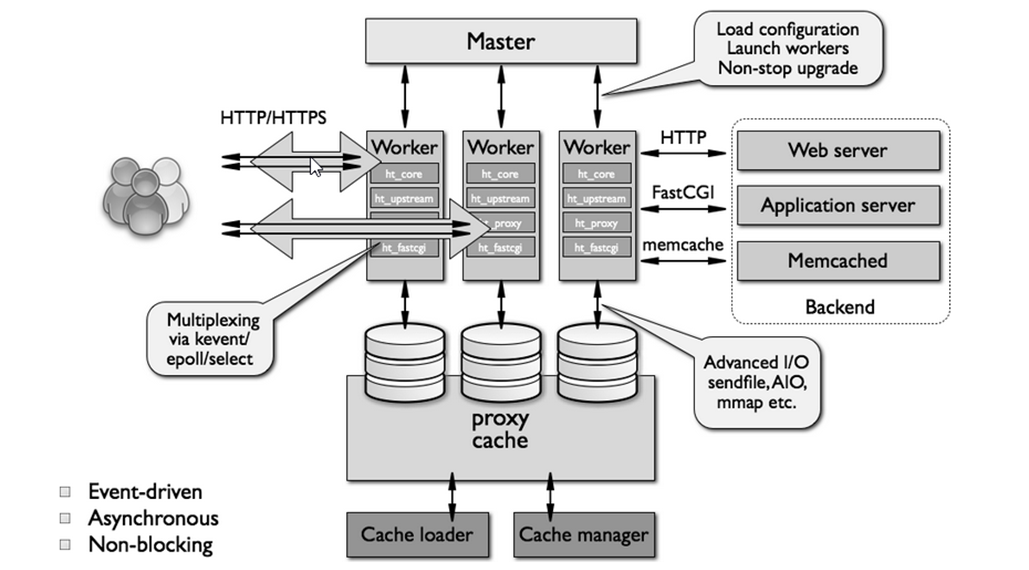
\includegraphics[scale=1]{figuras/nginx-how-it-works} 
\caption{Modelo de funcionamento do Nginx.}
\label{fig:nginx-comofunciona}
\end{figure}

O Nginx é utilizado por vários sítios de grande volume de tráfego como Netflix, GitHub, Pinterest, dentre outros.\\

\section{ApacheBench}
O ApacheBench foi criado em 1996 por Adam Twiss e, posteriormente doado ao Apache \textit{Group}. Originalmente, essa ferramenta foi desenvolvida para verificar o desempenho em servidores HTTP Apache, mas hoje ela é utilizada para fazer testes de desempenho em  praticamente qualquer servidor HTTP.

\section{FastCGI}
De acordo com \citeonline{fastcgi} FastCGI é uma interface para servidores \textit{web} rápida, aberta e segura, que resolve os problemas de desempenho herdados do CGI, sem introduzir o \textit{overhead} e complexidade de APIs proprietárias.

\subsection{\textit{Common Gateway Interface}}
A interface de fato de aplicações em servidores \textit{web} é o CGI, que foi primeiramente implementado no servidor da NCSA. O CGI tem muitos benefícios:

\begin{itemize}
	\item Simplicidade: é fácil de entender;
	\item Independente de linguagem: Aplicações em CGI podem ser escritas em quase todas a linguagens;
	\item Isolamento do processo: Com os processos são executados em processos separados, aplicações com problemas não podem para o servidor \textit{web} ou acessar o estado interno do servidor;
	\item Padrão aberto: Alguma forma de CGI já foi implementado em todos os servidores;
	\item Independência de arquitetura: O CGI não é ligado a uma arquitetura de computador em particular.
\end{itemize}

CGI tem alguns inconvenientes significantes. O principal problema é desempenho: como um novo processo é criado para cada requisição e descartada quando a requisição acaba,a eficiência é baixa.

\subsection{Servidor de API}
Em resposta ao problema de desempenho do CGI, várias empresas desenvolveram API's para os seus servidores.\\
Aplicações conectadas em um servidor de API pode ser significativamente mais rápido do que programas em CGI. O problema da inicialização do CGI é melhorada, pois a aplicação é executada no processo do servidor e persiste pelas requisições. As API's dos servidores \textit{web} também oferecem mais funcionalidades do que o CGI. O desenvolvedor pode criar extensões que permitem realizar controle de acesso, pegar um acesso dos aquivos de registro(\textit{log}) do servidor e, se conectar a outros estágios do processamento de uma requisição do servidor.\\
No entanto, API's sacrificam todos os benefícios do GCI. São eles:
\begin{itemize}
	\item Complexidade: API's de empresas introduzem uma curva de aprendizado, com curtos de implementação e manutenção maiores;
	\item Dependencia de linguagem: as aplicações devem ser escritas na linguagem suportada pelo desenvolvedor da API;
	\item Não há isolamento de processos: como o processo é executado dentro do endereçamento de memória do servidor, aplicações com problemas podem corromper o núcleo do servidor, comprometer a segurança e problemas no núcleo do servidor podem corromper as aplicações;
	\item Proprietário: Codificar a aplicação para uma determinada API força o desenvolvedor a utilizar aquele servidor em particular;
	Arquiteturas de computador iguais: As aplicações tem que compartilhar sa mesma arquitetura do servidor \textit{web}.

\end{itemize}

\subsection{FastCGI}
A interface do FastCGI combina os melhores aspectos do CGI e das API's proprietárias. Assim como o CGI, o FastCGI executa os processos de forma separada e isolada. As vantagens do FastCGI incluem:

\begin{itemize}
	\item Desempenho: Os processos do FastCGI são persistentes. Eles são reutilizados para manipular várias requisições. Isso resolve o problema de criar um novo processo para cada requisição;
	\item Simplicidade com fácil migração do CGI: a biblioteca de aplicação do FastCGI simplifica a migração de aplicações existentes feitas usando CGI. Aplicações feitas utilizando a biblioteca de aplicações do FastCGI podem ser executadas como programa CGI;
	\item Independente de linguagem: Assim como o CGI, as aplicações FastCGI podem ser escritas em qualquer linguagem;
	\item Isolamento de processos: Uma aplicação com problemas não pode corromper o núcleo do servidor ou de outra aplicação. Uma aplicação maliciosa não pode roubar informações do servidor \textit{web};
	\item Independência de arquitetura: O FastCGI não é ligado a uma arquitetura de computador em particular. Qualquer servidor \textit{web} pode implementar a interface do FastCGI;
	\item Suporte à computação distribuída: FastCGI provê a habilidade de executar aplicações remotamente, o que é útil para distribuir carga e gerenciar sítios da \textit{web} externos
\end{itemize}

\section{PHP}
Escrever sobre
\subsection{PHP-FPM}
Escrever sobre
\section{PostgreSQL}
Escrever sobre
\section{VirtualBox}
Escrever sobre
\section{Debian}
Escrever sobre